\documentclass[12pt,a4paper,titlepage]{article}
\usepackage[ngerman]{babel}
\usepackage[scale=0.8]{geometry}
\usepackage{amsmath}
\usepackage{amssymb}
\usepackage{setspace}
\usepackage{esint}
\usepackage{cancel}
\usepackage{units}
\usepackage{listings}
\usepackage{dsfont}
\usepackage{float}
\usepackage{morefloats}
\usepackage{fancyhdr}
\usepackage[utf8]{inputenc}
\usepackage{pdfpages}
\usepackage{siunitx}
\usepackage{wasysym}
\pagestyle{fancy}
\usepackage{marvosym}
\usepackage{eurosym}
\usepackage{graphicx}
\usepackage{url}
\setlength{\headheight}{15pt}
\setcounter{tocdepth}{5}
\setcounter{secnumdepth}{5}
\usepackage{hyperref}
\usepackage{csquotes}

\usepackage{graphicx}
\usepackage{tabularx}

\author{Jonas Rieder, Marcel Nitsch}
\date{\today}
\title{P521: $\gamma$-Spektroskopie mit Szintillations- und Halbleiterdetektoren}

\begin{document}

\section{Auswertung}

Alle Spektren wurden zuerst um die dazugehörigen Untergründe bereinigt, indem die Daten der Untegrundmessungen von denen der Spektren abgezogen wurden.

\subsection{Energiekalibrierung}

\subsubsection{Szintillator}

Zur Energiekalibrierung haben wir an die in den Spektren erkennbaren Ausschlägen Gaußfunktionen der Form
\begin{equation}
g(x) = \frac{a}{\sqrt{2\pi\sigma^2}}\exp{\frac{\left(x-\mu\right)^2}{2\sigma^2}} + cx + b
\end{equation}
angepasst. Aus den Werten für $\mu$ ergeben sich die Mittelwerte der Linien, die dann den Referenzspektren aus dem Versuchsheft und der Internetseite \ref{gammaspectacular} zugeordnet wurden. In Abbildung \ref{fig:sz_bsp} ist ein Beispiel für die Anpassung, die restlichen sind im Anhang \ref{an:sz_peaks}. In Tabelle \ref{tab:sz_kalib} sind die Mittelwerte der Anpassungen sowie die zugeordneten Linien.

\begin{figure}
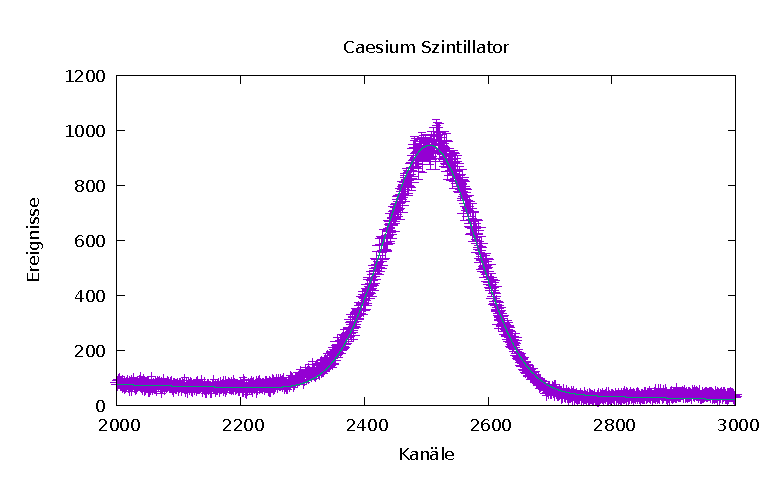
\includegraphics{caesium_sz}
\caption{Beispiel Gaußanpassung an das Caesium Spektrum (Szintillator)}
\label{fig:sz_bsp}
\end{figure}

\begin{table}
\centering
\begin{tabular}{c|c|c}
$\mu$ & $\Delta \mu$ & Linie in $\si{\kilo\electronvolt}$\\
\hline
$\num{2506.1}$&$\num{0.4}$&Caesium $\num{661.6}$\\
\hline
$\num{4399.4}$&$\num{0.8}$&Cobalt $\num{1173.2}$\\
$\num{4989}$&$\num{0.7}$&Cobalt $\num{1332.5}$\\
\hline
$\num{943.9}$&$\num{0.9}$&Europium $\num{964.06}$\\
$\num{1324.4}$&$\num{0.5}$&Europium $\num{344.3}$\\
$\num{3620}$&$\num{3}$&Europium $\num{964.06}$\\
\end{tabular}
\caption{Werte für die Kalibration beim Szintillator}
\label{tab:sz_kalib}
\end{table}

Die Werte der Mittelwerte wurden dann gegen die Energien der zugeordneten Linien aufgetragen und eine Gerade der Form
\begin{equation}
K(E) = mE + b
\end{equation}
daran angepasst. Daraus ergibt sich
\begin{eqnarray}
m &=& \left(\num{3.7}\pm\num{0.01}\right)\si{\kilo\electronvolt^{-1}}\\
b &=& \num{47}\pm\num{5}\ .
\end{eqnarray}
Dies ist in Abbildung \ref{fig:sz_kalib} dargestellt. Auf Grund der großen Anzahl an Messwerten sind die Fehler auf die Mittelwerte sehr klein. Dies führt bei der Anpassung zu einem sehr hohen $\chi^2$ Wert. Er liegt bei dieser Anpassung bei $\num{65.3}$. Mit Hilfe dieser Kalibrationsfunktion, bzw. ihrer Umkehrung, konnten dann die Spektren in Abhängigkeit von der Energie dargestellt werden. Die Spektren sind in den Abbildungen \ref{fig:cs_sz}, \ref{fig:co_sz} und \ref{fig:eu_sz} dargestellt.
\begin{figure}
	\centering
	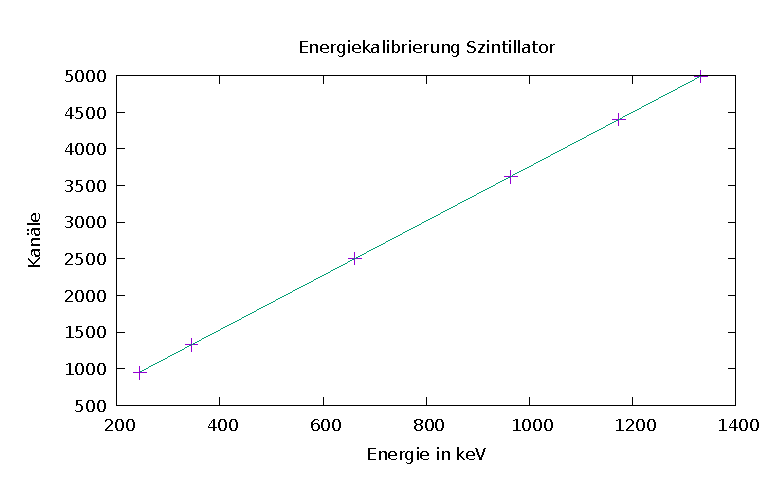
\includegraphics{kalib_sz}
	\caption{Kalibrationskurve Szintillator}
	\label{fig:sz_kalib}
\end{figure}
\begin{figure}
	\centering
	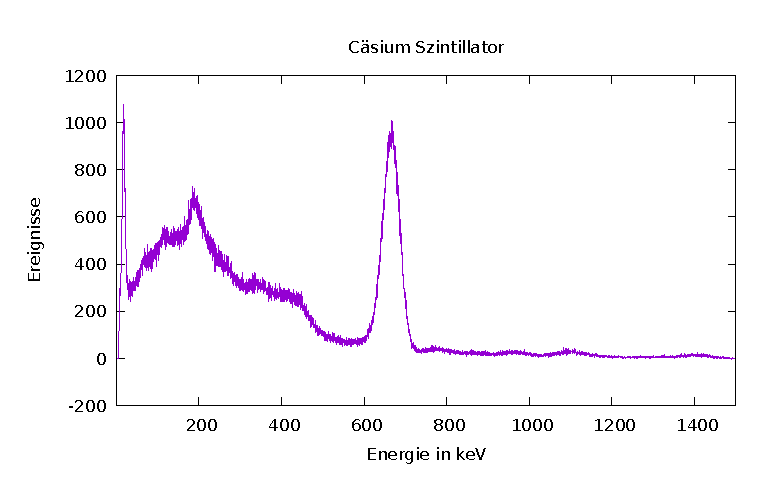
\includegraphics{caesium_sz_energie}
	\caption{Caesiumspektrum Szintillator}
	\label{fig:cs_sz}
\end{figure}
\begin{figure}
	\centering
	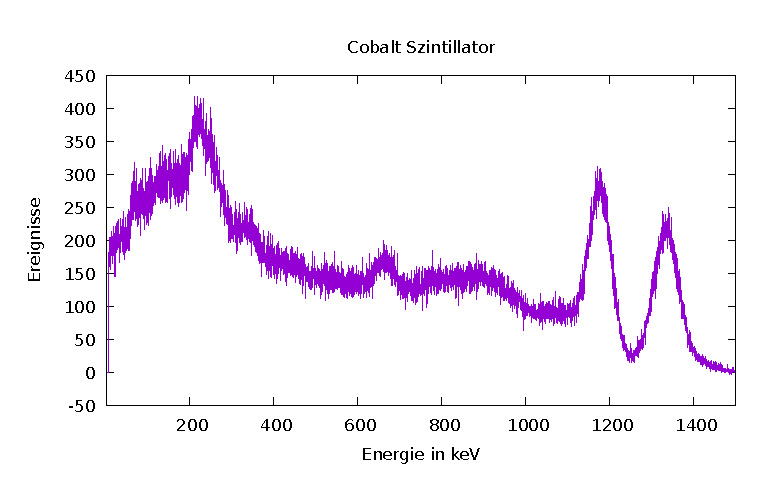
\includegraphics{cobalt_sz_energie}
	\caption{Cobaltspektrum Szintillator}
	\label{fig:co_sz}
\end{figure}
\begin{figure}
	\centering
	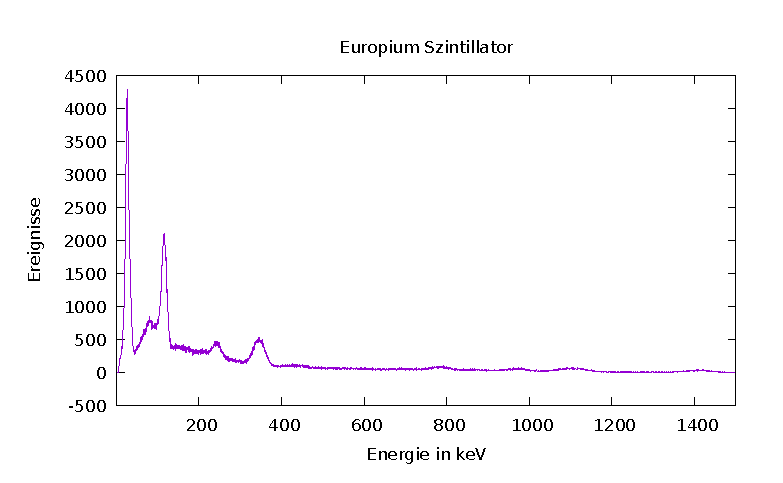
\includegraphics{europium_sz_energie}
	\caption{Europiumspektrum Szintillator}
	\label{fig:eu_sz}
\end{figure}

\subsubsection{Halbleiter}
Bei der Kalibrierung wurde ebenso vorgegangen, wie beim Szintillator. Da hierbei jedoch die Linien deutlich schärfer aufgelöst sind, konnten beim Europium Spektrum deutlich mehr zur Kalibration verwendet werden.


\end{document}
